\documentclass[12pt]{standalone}

\usepackage{pgfplots} 
\usetikzlibrary{patterns}
%\usepackage[dvipsnames]{xcolor}
\usepackage{colortbl}

\definecolor{c0}{HTML}{C16E71}
\definecolor{c1}{HTML}{E5A79A}

\definecolor{c2}{HTML}{D0D08A}
\definecolor{c3}{HTML}{7DA494}
\definecolor{c4}{HTML}{ABC8E5}
\definecolor{c5}{HTML}{6E8FB2}
\definecolor{c6}{HTML}{9F8DB8}

\begin{document}
    \begin{LARGE}
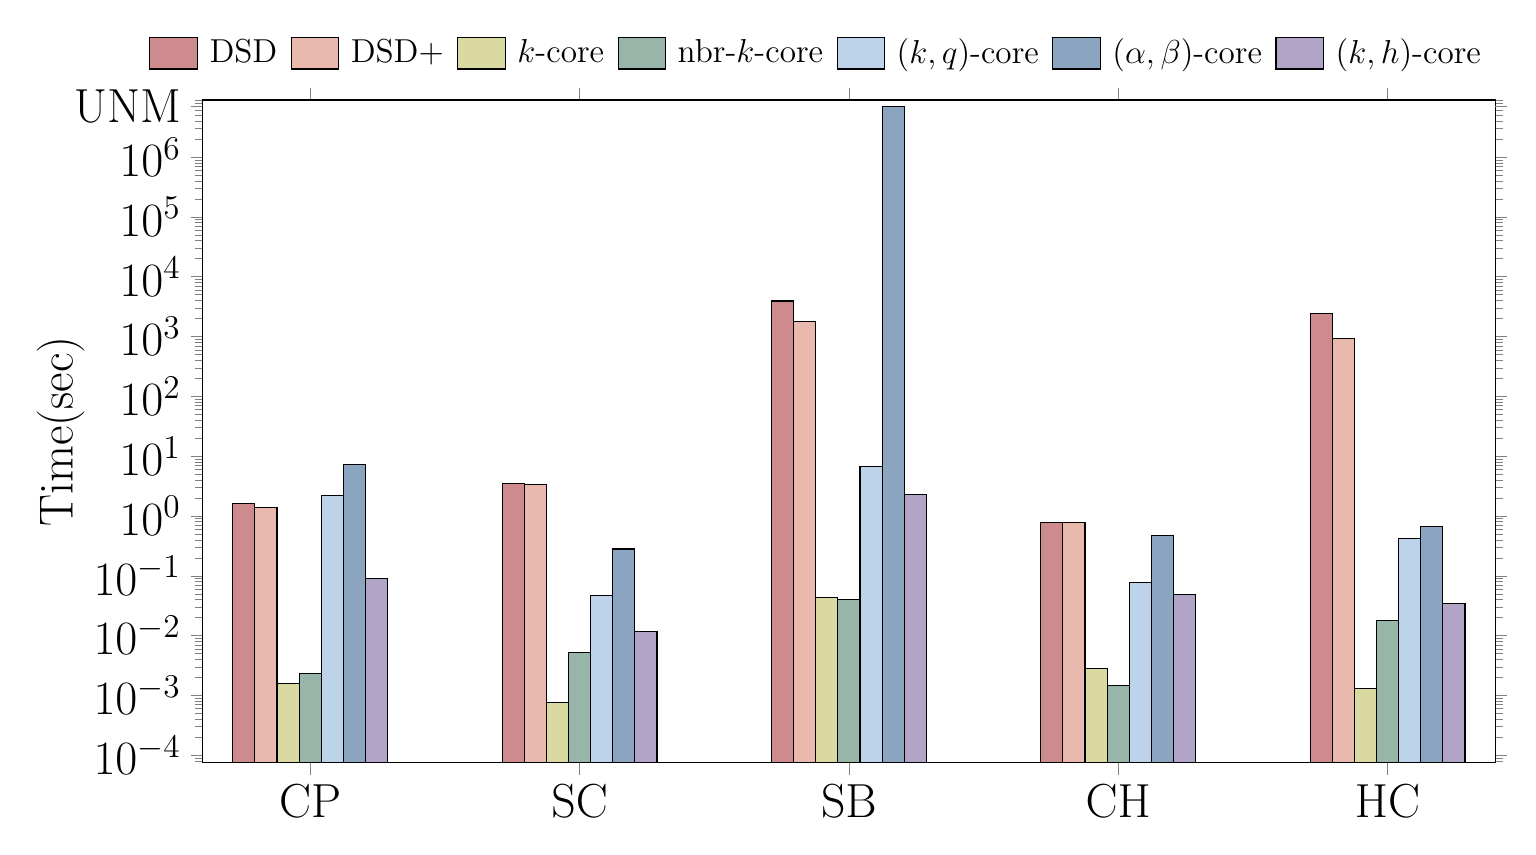
\begin{tikzpicture}
\begin{axis}
[
    width=18cm,
    height=10cm,
    ymode=log,
    ymax=9000000,
    %ymin=0.001, % 确保最小值是正值
    %ymax=37,
    log origin=infty, % 将柱子从 x 轴起绘制
    ybar=0pt, 
    extra y ticks={7000000},
    extra y tick style={
        yticklabel={UNM}    
    },
    bar width=8pt,
    tick align=outside,
    ylabel near ticks, 
    ylabel shift={-15pt},
    xlabel near ticks, 
    xlabel shift={-2pt},
    legend columns=8, 
    column sep=2.5cm,
    legend image code/.code={%
                    \draw[#1, draw=black] (0cm,-0.2cm) rectangle (0.6cm,0.2cm);
               }, 
    legend style={draw=none,font=\large, at={(1,1.11)},%anchor=north, 
        /tikz/every even column/.append style={column sep=0.1cm},
        /tikz/every odd column/.append style={column sep=0.08cm}},
    font=\LARGE, 
    ylabel={Time(sec)}, 
    %xlabel={$\delta$},
    symbolic x coords={CP,SC,SB,CH,HC}, 
    xtick=data, 
]

\addplot [fill=c0!80] coordinates {(CP, 1.6033) (SC, 3.44832) (SB, 3928) (CH, 0.77540)(HC,2404.01)}; 
\addplot [fill=c1!80] coordinates {(CP, 1.39902) (SC, 3.36347) (SB, 1768.51) (CH,0.786885)(HC,929.404)};
%k-core
\addplot [fill=c2!80] coordinates {(CP, 0.001562) (SC, 0.000757) (SB, 0.043665) (CH,0.002812)(HC,0.001289)};
%nbr-kcore
\addplot [fill=c3!80]  coordinates {(CP, 0.002357) (SC, 0.005183) (SB, 0.040527) (CH,0.001457)(HC,0.01783)};
%kqcore
\addplot [fill=c4!80] coordinates {(CP, 2.18968) (SC, 0.046636) (SB, 6.67124) (CH,0.078176)(HC,0.420761)};
%abcore
\addplot [fill=c5!80] coordinates {(CP, 7.16514) (SC, 0.280068) (SB, 7000000) (CH,0.474329)(HC,0.658944)};
%khcore
\addplot [fill=c6!80] coordinates {(CP, 0.089597) (SC, 0.011824) (SB, 2.28328) (CH,0.049475)(HC,0.034562)};


%https://tikz.dev/library-patterns
\legend{DSD, DSD+,$k$-core, nbr-$k$-core, ($k, q$)-core, ($\alpha,\beta$)-core, ($k, h$)-core}

\end{axis}
\end{tikzpicture}
\end{LARGE}
\end{document}


\addplot [pattern=north east lines, pattern color=c1] coordinates {(CP, 1.6033) (SC, 3.44832) (SB, 3928) (CH, 0.77540)(HC,2404.01)(HB,100000)(WT,100000)(TC,100000)}; 
\addplot [pattern=grid, pattern color=c3] coordinates {(CP, 1.39902) (SC, 3.36347) (SB, 1768.51) (CH,0.786885)(HC,929.404)(HB,343)(WT,188)(TC,643)};
